\newpage
\section{Filter\hartl{509}}
\subsection{Tiefpass-Filter\hartl{514}}

\begin{longtable}{|>{\bfseries}p{3cm}|c|p{10cm}|}
    \hline
    1. Ordnung
    & 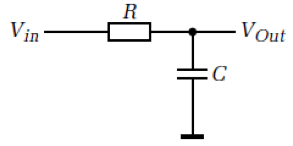
\includegraphics[width=4cm, valign=t]{pictures/tiefpass1ordnung}
    & {\textbf{UTF: } $G(s): \frac{1}{1+s C\cdot R} = \frac{1}{1+ j\cdot \frac{\omega}{\omega_{3dB}}}$\newline
        $f_{3dB}=\frac{1}{2\pi R\cdot C}$\newline
        Bei $j\omega=\frac{1}{T}$ sind Real- und Imaginärteil gleich gross: $T=\frac{1}{R \cdot C}$
      }
    \\ \hline
% ----------------------------------------------------------------------------------------------------    
    {2. Ordnung\newline
     (kaskadierte RC-Tiefpässe)
    }
    & 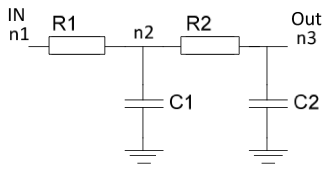
\includegraphics[width=4cm, valign=t]{pictures/tiefpass2ordnung}
    & {Stromgleichungen für Knoten $n_2$ und $n_3$ (out)\newline
       $0=(U_{n2}-U_{in})\cdot \frac{1}{R_1}+(U_{n2}-U_{n3})\cdot \frac{1}{R_2}+U_2\cdot s C_1$\newline
       $0=(U_{n3}-U_{n2})\cdot \frac{1}{R_2}+U_{n3}\cdot s C_2$\newline
       $G_{p}(s)= \frac{U_{out}}{U_{in}} = \frac{1}{C_1\cdot C_2\cdot R_1\cdot R_2\cdot s^2+ (C_1\cdot R_1 + C_2\cdot R_1 + C_2\cdot R_2)\cdot s+1}$\newline\newline
       Vgl. allgemeiner Tiefpass 2. Ordnung:\newline
       \begin{align*}
           G_{LP}(s)	&= \frac{A0}{\frac{s^2}{\omega_{0}^2}+\frac{s}{Q\cdot\omega_{0}}+1} \\
           A0	 		&= 1 \\
           \omega_{0}	&= \frac{1}{\sqrt{C_1\cdot C_2\cdot R_1\cdot R_2}}\\
           Q 	        &=\frac{\sqrt{C_1\cdot C_2\cdot R_1\cdot R_2}}{R_1\cdot (C_1+C_2)+C_2 \cdot R_2}
        \end{align*}\newline
        Passive RC-Filter können maximal Güte von 0.5 haben (2 identische reelle Pole) Filter höherer Güte benötigen Spulen oder Verstärker
      }
      \\ \hline
% ----------------------------------------------------------------------------------------------------      
    {Sallen Key\newline
     (Einfachmit-kopplung)\newline
     \hartl{517}
    }
    & 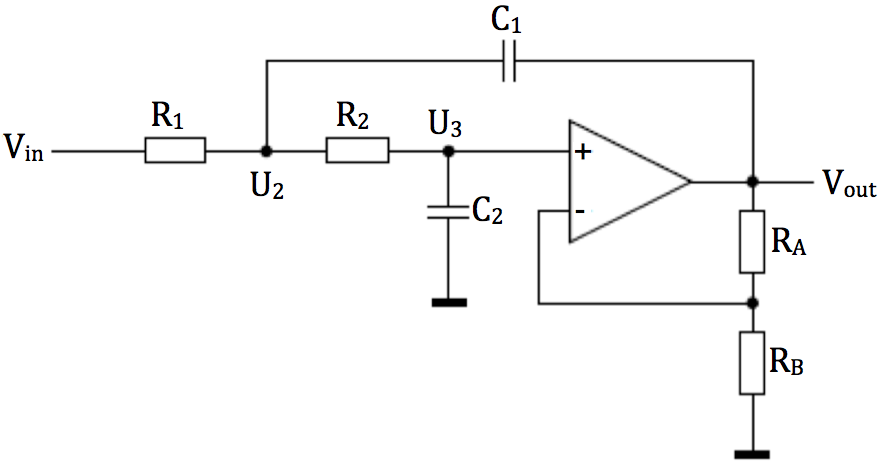
\includegraphics[width=4cm, valign=t]{./pictures/sallenkey.png}
    & {{\bf Standard Sallen Key}\newline
       Stromgleichungen:\newline
       $0 = (U_2-U_{in})\cdot \frac{1}{R_1}+(U_2-U_3)\cdot \frac{1}{R_2}+(U_2-U_{out})\cdot s C_1$ \newline
       $0 = (U_3-U_2)\cdot \frac{1}{R_2}+U_3\cdot s C_2$\newline
       Verstärkung:\newline
       $U_{out}=G_0\cdot U_3$ mit $G_0 = \frac{R_{A}+R_{B}}{R_{B}}$\newline
       \begin{align*}
           G_{SK}	&= \frac{G0}{C_1\cdot C_2\cdot R_1\cdot R_2\cdot s^2+[C_2\cdot (R_1+R_2)+C_1\cdot R_1\cdot (1-G_0)]\cdot s +1}\\
           \omega_0 &= \frac{1}{\sqrt{C_1\cdot C_2\cdot R_1\cdot R_2}}\\
           Q_{SK}	&= \frac{\sqrt{C_1\cdot C_2\cdot R_1\cdot R_2}}{C_2\cdot (R_1+R_2)+C_1\cdot R_1\cdot (1-G_0)}
       \end{align*}
      }
    \\
    & 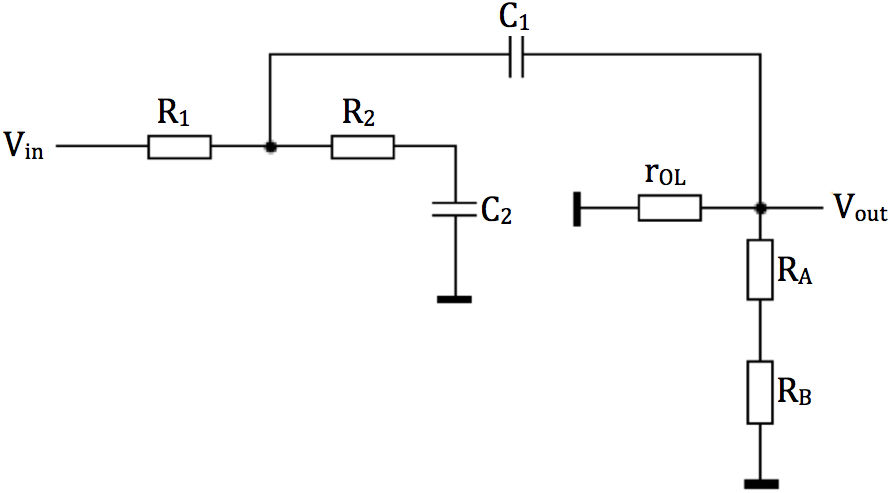
\includegraphics[width=4cm, valign=t]{./pictures/sallenkey2.png}
    & {{\bf für hohe Frequenzen}\newline
        \vspace{-1.5\topsep}
        \begin{itemize}[leftmargin=*]
            \item Wenn der Opamp nicht mehr verstärkt
            \item $C_1$, $C_2$ wirken als Kurzschlüsse
            \begin{equation*}
                \frac{V_{Out}}{V_{in}}=\frac{r_{OL}\parallel R_2\parallel
                    (R_{A}+R_{B})}{R_1+r_{OL}\parallel R_2\parallel (R_{A}+R_{B})}\approx
                \frac{r_{OL}}{R_1+r_{OL}}
            \end{equation*}
            \item Folge: Sallen Key-Filter sind nicht geeignet für Systeme mit hohen
            Frequenzanteilen, z.B. PEM-DAC
        \end{itemize}   
      }
      \\ \hline
% ---------------------------------------------------------------------------------------------------- 
      {Multiple Feedback\newline
       \hartl{522}
      }
      & 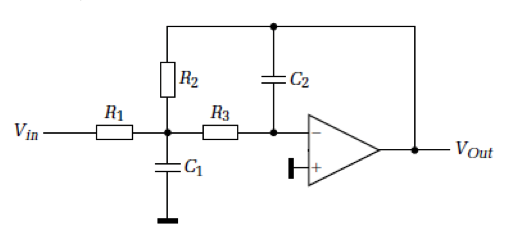
\includegraphics[width=4cm, valign=t]{./pictures/mulipleFeedback.png}
      & {Stromgleichungen: (Opamp sorgt für $U_3=0$)\newline
         $0	=(U_2-U_{in})\cdot \frac{1}{R_1}+(U_2-U_{out})\cdot \frac{1}{R_2}+(U_2-U_3)\cdot \frac{1}{R_3}+U_2\cdot s C_1$\newline
         $0	=(U_3-U_2)\cdot \frac{1}{R_3}+(U_3-U_{out})\cdot s C_2$\newline\newline
         $G_{mf}(s)	=\frac{G_0}{1+C_2(R_2+R_3+R_3\cdot \frac{R_2}{R_1})\cdot s+C_1\cdot C_2\cdot R_2\cdot R_3\cdot s^2}$ mit $ G_0 = -\frac{R_2}{R_1}$\newline
         $Q_{mf} =\frac{\sqrt{C_1\cdot C_2\cdot R_2\cdot R_3}}{C_2\cdot (R_2+R_3+R_3\cdot \frac{R_2}{R_1})}$\newline
         Die Güte wird v.a. eingestellt mit $C_2$ und $R_1$, grosse Güte für kleines $C_2$ und grosses $R_1$. $C_2$ beeinflusst auch das Frequenzverhalten, $R_1$ die Verstärkung.
        }
      \\ \hline
% ---------------------------------------------------------------------------------------------------- 
      {Zustandsvariab-len-Filter
      }
      & 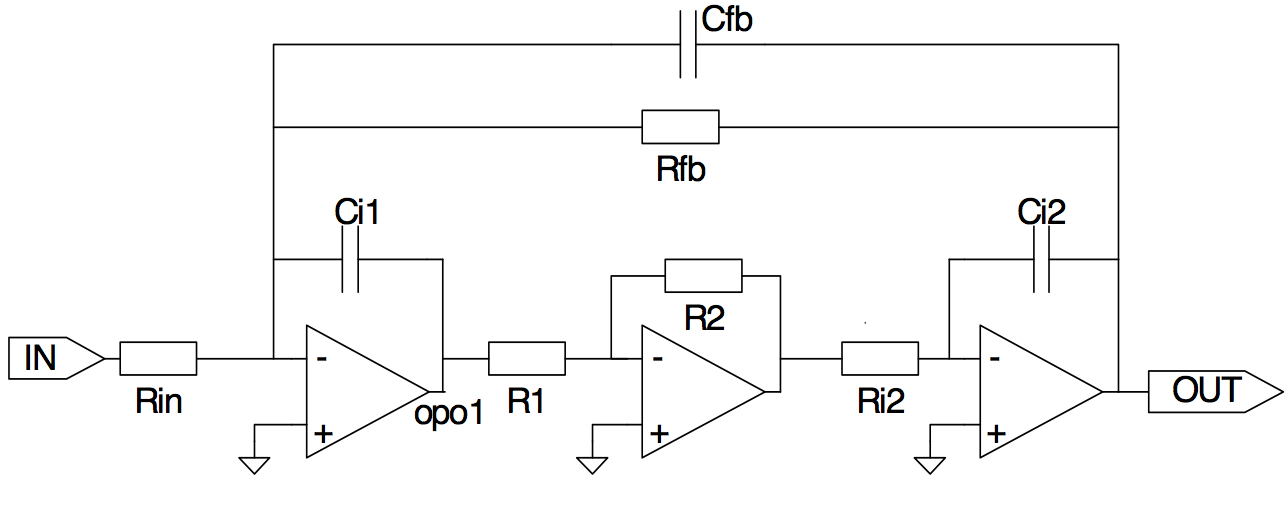
\includegraphics[width=4cm, valign=t]{./pictures/zustandsvariable.png}
      & {Spannungsgleichungen:\newline
         \begin{align*}
             V{out}		&=-\frac{1}{s C_{i2}\cdot R_{i1}}\cdot V_{opo2}\\
             V_{opo2}	&=-\frac{R_2}{R_1}\cdot V_{opo1}\\
             V_{opo1}	&=\frac{-1}{s C_{i1}}\cdot (\frac{V_{in}}{R_{in}}+\frac{V_{out}}{R_{fb}}+s C_{fb}\cdot V_{out})\\
             G_{ss}(s)	&=\frac{-\frac{R_{fb}}{R_{in}}}{C_{i1}\cdot C_{i2}\cdot R_{i1}\cdot R_{fb}\cdot \frac{R_1}{R_2}\cdot s^2+C_{fb}\cdot R_{fb}\cdot s+1}\\
             A_{0}		&=-\frac{R_{fb}}{R_{in}}\\
             \omega_{0}	&=\frac{1}{\sqrt{C_{i1}\cdot C_{i2}\cdot R_{i1}\cdot R_{fb}\cdot \frac{R_1}{R_2}}}\\
             Q			&=\frac{\sqrt{C_{i1}\cdot C_{i2}\cdot R_{i2}\cdot \frac{R_1}{R_{fb}\cdot R_2}}}{C_{fb}}
         \end{align*}
         D.h. mit dieser Topologie sind alle 3 Parameter frei wählbar!
         \begin{enumerate}
             \item $\omega_{0}$ mit $C_{i1}$, $C_{i2}$, $R_{fb}$, $R_{i2}$, $R_1$, $R_2$
             \item Q mit $C_{fb}$
             \item $A_0$ mit $R_{in}$
         \end{enumerate}
        }
      \\ \hline
\end{longtable}


